
\FloatBarrier
\begin{figure}[h!]
    \centering
    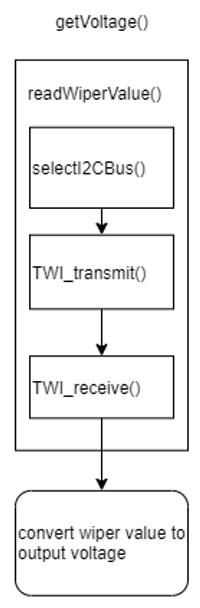
\includegraphics[scale=0.7]{software_getVoltage_flow_chart.png}
    \caption{Flow chart of the getVoltage funcion.}
    \label{fig:getvoltage}
\end{figure}
\FloatBarrier
\begin{figure}[h!]
    \centering
    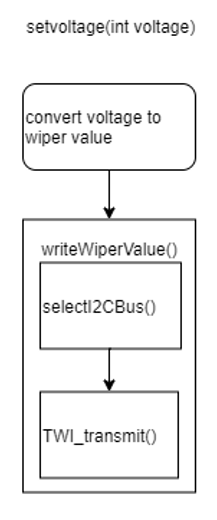
\includegraphics[scale=0.7]{software_setVoltage_flow_chart.png}
    \caption{Flow chart of the setVoltage funcion.}
    \label{fig:setvoltage}
\end{figure}
\FloatBarrier
\begin{figure}[h!]
    \centering
    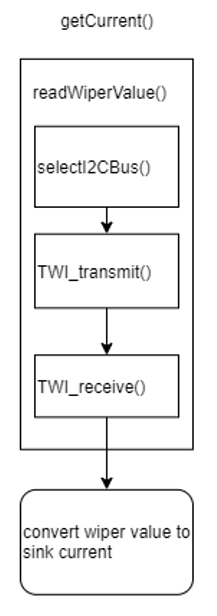
\includegraphics[scale=0.7]{software_getCurrent_flow_chart.png}
    \caption{Flow chart of the getCurrent funcion.}
    \label{fig:getcurrent}
\end{figure}
\FloatBarrier
\begin{figure}[h!]
    \centering
    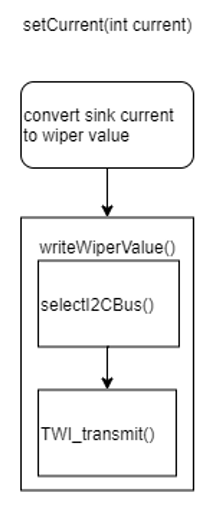
\includegraphics[scale=0.7]{software_setCurrent_flow_chart.png}
    \caption{Flow chart of the setCurrent funcion.}
    \label{fig:setcurrent}
\end{figure}
\FloatBarrier